\section{Setup and procedure}
\paragraph{The experiment consists}
of six separate steps, each with a different setup and goal. 
We give an overview of this program and link the corresponding circuits to 
each point. Thereafter we add a few comments on the setup. 
\begin{enumerate}
    \item 
        \textbf{Assessing the detectors and probe at hand with the oscilloscope:}
        We measure the signals of the preamplifier (PA) as wel as uni- and bipolar outputs of 
        main amplifier (MA) at the oscilloscope. With this signal, we calculate the ascending time 
        of the signal.
    \item 
        \label{it:task2}
        \textbf{Recording the energy spectrum of$\, ^{57}$Co and $^{241}$Am:}
        The multichannel analyzer (MA) we measure the energy spectrum of both probes 
        for ca. 10 minutes. With the $^{57}$Co sample, we test the sensibility of each detector
        and the optimal positioning of the sample (which is not symmetric). 
        The used circuit is shown in figure~\ref{fig:circuit_spectrum}. After assigning the 
        channel-energy relationship based on the knowledge of some peaks, we interprete the other visible peaks.
    \item
        \textbf{Setting the energy windows:}
        In this step, we restrict the events passed by the single channel analyzer (SCA) to those 
        of the 14.4 keV and 122 keV photons, respectively. We use the circuit depicted in figure~\ref{fig:circuit_window}
    \item
        \textbf{Time calibration of Time to Amplitude converter (TAC):}
        In order to correlate measured channel and the respective time delay, we measure the channel 
        assigned by TAC and MCA corresponding to a known delay and perform a fit a linear function between 
        the two quantities. This correspondance will be used in the anaylsis of the delayed coincidences. 
        The corresponding circuit can be observed in figure~\ref{fig:circuit_calibrate}
    \item
        \textbf{Measuring the delayed coincidences:}
        Using the Time-to-Amplitude converter (TAC) as depicted in figure~\ref{fig:circuit_coincidences}, 
        we record the delays between 14.4 keV and 122 keV 
        events. Since the 14.4 keV photon is only emitted in 10 \% of the cases, we use this signal to start the 
        TAC, and stop with the delayed 122 keV photon, expecting to drastically reduce the dead time of the 
        measurement.
    \item
        \textbf{Measuring the background (random coincidences):}
        Taking out the delay of the 122 keV signal and further introducing a delay on the 14.4 keV signal, 
        we measure the background. 
\end{enumerate}

\begin{figure}[H]
    \centering
    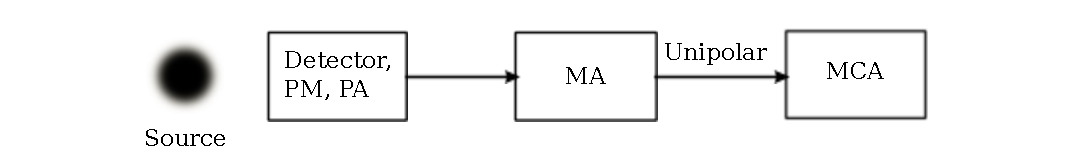
\includegraphics[width=\linewidth]{figures/circuit1.pdf}
    \caption{
        Scheme of the circuit used in the measurement of the energy spectra. 
        }
    \label{fig:circuit_spectrum}
\end{figure}

\begin{figure}[H]
    \centering
    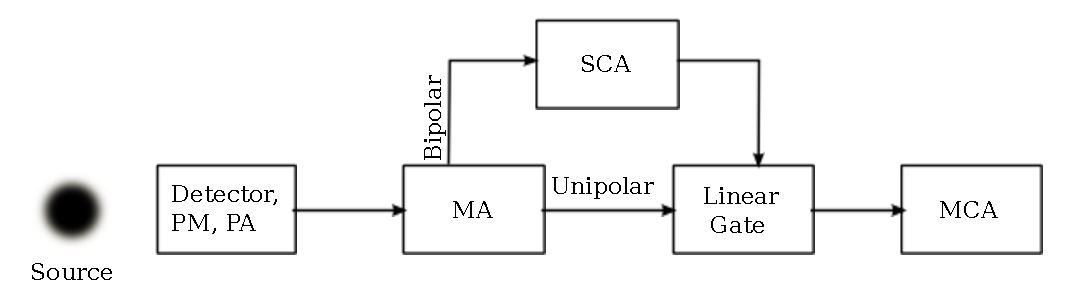
\includegraphics[width=\linewidth]{figures/circuit2.pdf}
    \caption{
        Scheme of the circuit used for setting the energy windows. 
        }
    \label{fig:circuit_window}
\end{figure}

\begin{figure}[h]
    \centering
    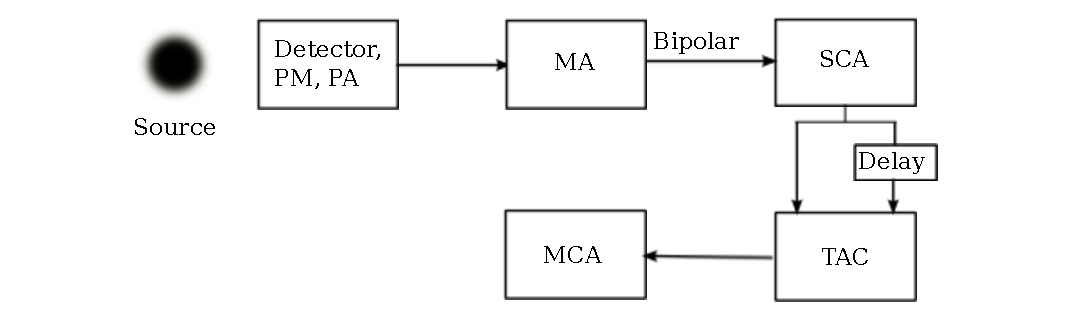
\includegraphics[width=\linewidth]{figures/circuit3.pdf}
    \caption{
        Circuit for calibration of TAC. The delay is changed to produce a 
        series of relations delay -- channel which will be used to do a 
        linear fit. 
        }
    \label{fig:circuit_calibrate}
\end{figure}

\begin{figure}[h]
    \centering
    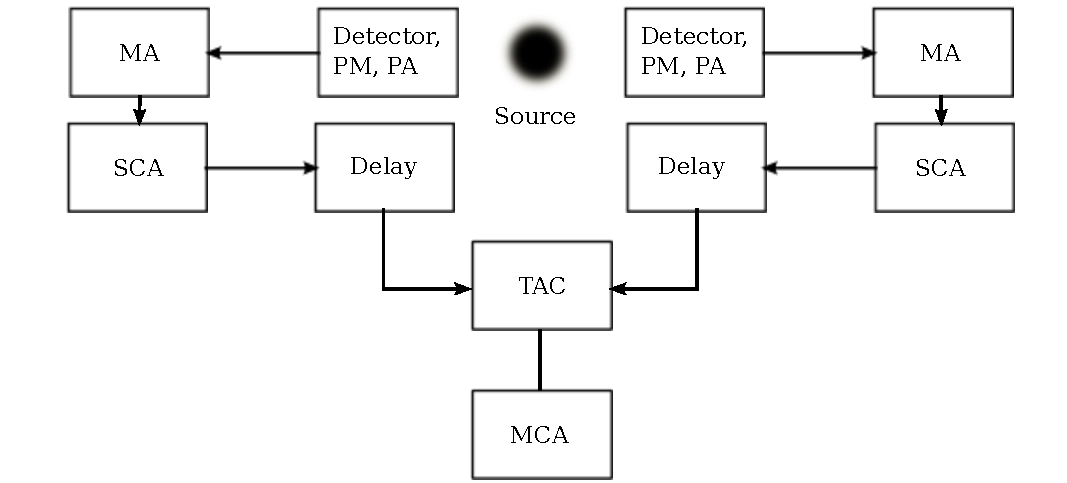
\includegraphics[width=\linewidth]{figures/circuit4.pdf}
    \caption{
        Scheme of the circuit used for measuring the delayed coincidences, 
        as well as the background (changes only in the applied delay). 
        }
    \label{fig:circuit_coincidences}
\end{figure}

\paragraph{The setup of the experiment}
consists of a fixed part with probe and a detector at each side 
as well as a part with the electronics. The devices are adapted to each part, as described below. 
A photo of the two detectors and the probe is shown in figure \ref{fig:position_1}. The given setup also 
defines position 1, later referred to as "Pos1" (see table \ref{tab:config2}). Position 2 ("Pos2") corresponds 
to the probe rotated by $180^\circ$. From its geometry, one can already suspect that the number of photons 
that can be measured from either direction is not equal. A similar condition is true for the detectors:
Already on the first glance, it is clear that the two are not of the same model. In fact, the left detector 
is an older model and suspected to be less sensitive. A more quantitative statement will be made in the 
of the second part of the experiment (see \ref{it:task2}). The detectors shown each include a photodiode 
and a pre-amplifier (PA). 
All further electronics are located on a 19 inch rack as shown in figure~\ref{fig:rack}.

\begin{figure}[h]
    \centering
    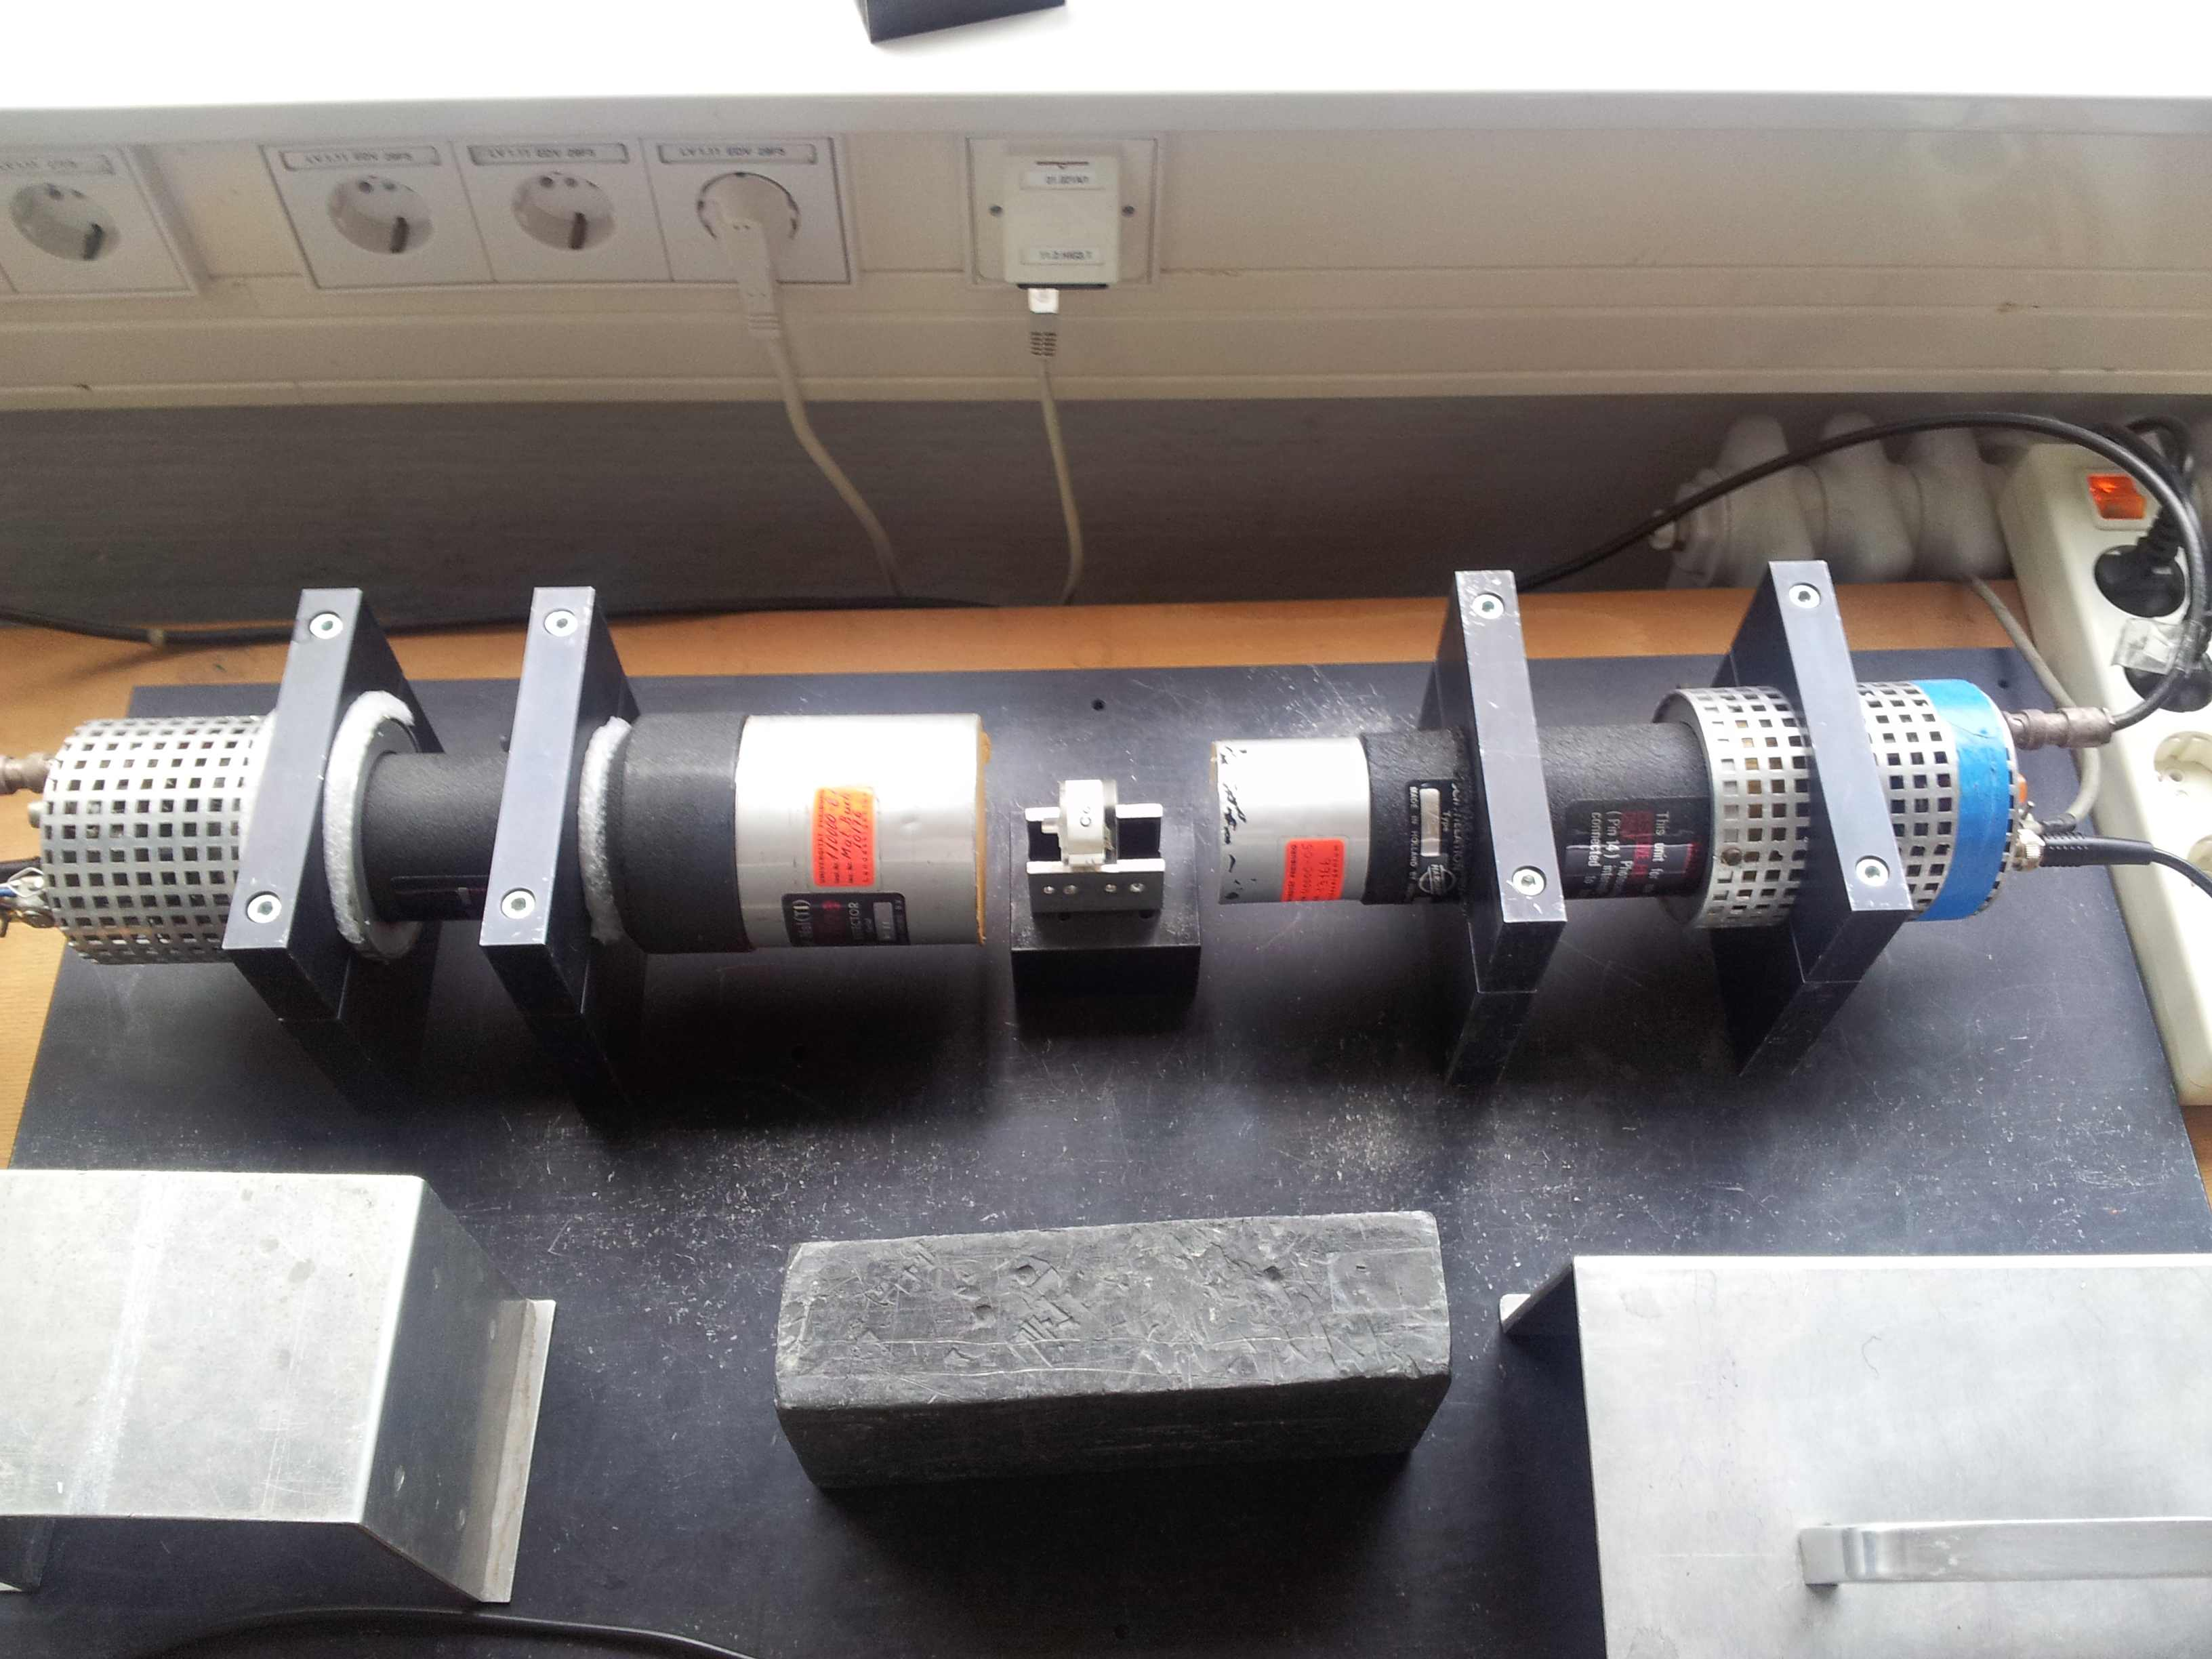
\includegraphics[width=0.8\linewidth]{figures/position_1.jpg}
    \caption{
        photo of the $^{57}$co probe and the two detectors with the setup used in the 
        experiment. the orientation of the probe is the one used for the measurement of 
        the delayed coincidences, with the larger opening facing the right detector. 
        during the measurements, the probe is isolated by the shields seen below the detectors.
        }
    \label{fig:position_1}
\end{figure}

\begin{figure}[H]
    \centering
    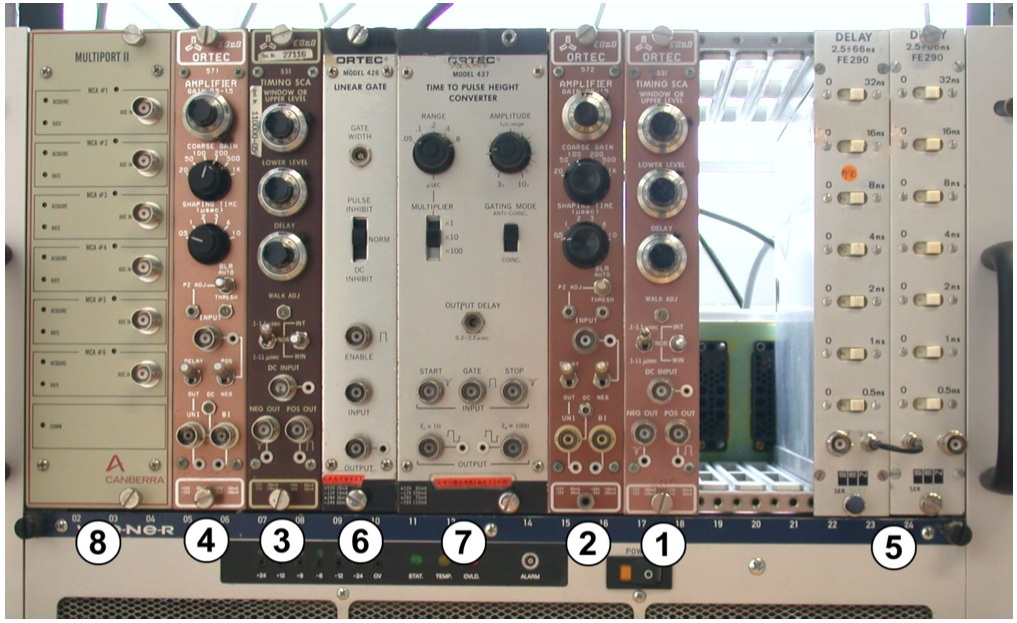
\includegraphics[width=0.8\linewidth]{figures/rack_anleitung.jpg}
    \caption{
        Photo of the rack with the electronic devices used in the experiment.
        The numbers correspond to: 
        (1) and (3) single channel analyzer (SCA);
        (2) and (4) main amplifier (MA);
        (5) delays;
        (6) linear gate;
        (7) time-to-amplitude converter (TAC);
        (8) multichannel analyzer (MCA).
        A third delay of the same kind not shown on the photo was used. 
        Taken from \cite{ver}.
        }
    \label{fig:rack}
\end{figure}



\FloatBarrier
